%
% General structure for the revdetua class:
%
\documentclass[shortpaper]{revdetua}
%
% Valid options are:
%
%   longpaper --------- \part and \tableofcontents defined
%   shortpaper -------- \part and \tableofcontents not defined (default)
%
%   english ----------- main language is English (default)
%   portugues --------- main language is Portuguese
%
%   draft ------------- draft version
%   final ------------- final version (default)
%
%   times ------------- use times (postscript) fonts for text
%
%   mirror ------------ prints a mirror image of the paper (with dvips)
%
%   visiblelabels ----- \SL, \SN, \SP, \EL, \EN, etc. defined
%   invisiblelabels --- \SL, \SN, \SP, \EL, \EN, etc. not defined (default)
%
% Note: the final version should use the times fonts
% Note: the really final version should also use the mirror option
%

\usepackage{scicite}
\usepackage{hyperref}

\usepackage{amsmath}
\usepackage{multicol}
\usepackage{setspace}

\usepackage{enumitem}

\usepackage{graphicx}
\usepackage{caption}
\usepackage{float}
\usepackage{subcaption}

\usepackage{verbatim}

\begin{document}
 
\Header{1}{85122}{Novembro}{2019}{1}

\title{\LARGE{{\bf Project 1: Algorithm Development Strategies\/}}}

\author{
\Large{{\bf A Study on 'The Change-Making Problem'\/}}\\\\\\
Filipe Pires [85122]\\
\\
{\bf Advanced Algorithms\/}\\
\normalsize{Department of Electronics, Telecommunications and Informatics}\\
\normalsize{University of Aveiro}\\
} 

\maketitle

\begin{abstract}
It is widely known that many computationally-demanding problems require more 
efficient solutions than to simply search exaustively for the answers.
This is particularly true for tasks that execute repeated operations in 
considerable amounts of times.
In this report, I focus on a famous challenge called 'The Change-Making Problem' 
and present a study on the computational performance of dynamic programming 
algorithms for solving such problem.
The implemented algorithms were 3, and they all follow the same strategy to 
tackle the issue so that a high fidelity comparison could be analysed.
\end{abstract}

\begin{keywords}
Algorithm Complexity, 'The Change-Making Problem', Dynamic Programming, 
Memoization, Scalable Algorithms.
\end{keywords}

\section*{1. Problem Contextualization}

This report was written for the course of 'Advanced Algorithms', taught by 
professor Joaquim Madeira for the master's in Informatics Engineering at DETI UA.
It describes the work done for the first assignment of the course \cite{trab1},
aimed to elaborate a study on the complexity and performance of algorithms that
solve one of the proposed challenges.
The chosen hypothesis for the study was 'B - Dynamic Programming', and the chosen
problem was 'The Change-Making Problem' (hereafter referred to by tCMP).

The basic idea behind tCMP is to find the minimum number of coins, from a given 
set of coins of different values, that add up to a given amount of money.
To simplify the problem, it is usually assumed that for each possible coin value
there is an infinite amount of coins available to return the change.
This challenge quickly becomes computationally-demanding when the amount to 
return as change increases, considering a limited number of available coin 
alternatives.

TCMP is considered a special case of 'The Knapsack Problem' \cite{mit}, if 
the change amount is mapped to the knapsack's maximum weight and the chosen 
coins mapped to the weights of the items to be inserted into the knapsack.
In this specialization, the chosen coins must add up to exactly the knapsack's
maximum weight. 

The problem's applications are wider than just currency; another famous example 
is 'The 9 Dard Finish Problem', where the aim is to find out how can one dart 
player get a perfect leg using the fewest amount of darts possible (which is 9)
to sum a total of 501 points \cite{9df}.
However,to keep my study focused, I do not consider any other application.

TCMP is also the most common variation of 'The Coin Change Problem' \cite{g4g},
where the aim is to  find out the number of possible ways of making a change for
a given amount, without considering the coins order and considering the infinite
set of coin alternatives previously mentioned. 


\section*{2. Implementations}

In this chapter I present the mathematical definition of the problem and a
description of the three chosen algorithms for solving it.

To simplify the mathematical operations, I only consider positive integer values
for the coins and change amounts.
With this in mind, the coin values can be modeled by a set of {\it n\/} distinct 
values, arranged in increasing order as $a_1$ through $a_n$, and the 
problem by: given an amount $A$, how to find a set of integers 
$\{ x_1, x_2, ..., x_n\}$, with each $x_j$ representing how often the coin 
with value $a_j$ is used, which minimize the total number of coins 
$f(A)$, given by equation \ref{eq:1}, subject to equation \ref{eq:2}.
{\setstretch{0.1}
    \begin{multicols}{2}
        \begin{equation} \label{eq:1}
            f(A) = \sum_{j=1}^{n} x_j
        \end{equation}
        \break
        \begin{equation} \label{eq:2}
            A = \sum_{j=1}^{n} a_j x_j
        \end{equation}
    \end{multicols}
}

When planning the implementation of the algorithms to solve tCMP, I looked for
returning not only the minimum number of coins needed to add up to a given 
amount, but also the list of those same coins.
This would force me to develop a more complete solution and would help me 
manually check for the validity of the results during the development phase 
and better compare results between algorithms.

The first implemented algorithm resorted to a recursive function.
This function, {\it tCMP\_recursive()\/}, accepts as arguments the amount to be
given as change and a list containing the currency available, i.e. the coin 
alternatives to use when giving the change.
The way it works is by iterating over the available coins (from the end to the 
beginning, i.e. from the highest coin to the lowest), comparing the results 
of using the current coin or using the next one and returning the best alternative.
The function keeps track of the currently used coin with the help of an auxiliar
function that receives the current index of the currency list as an argument; it
is this function {\it tCMP\_recursive\_getMinCurrency()\/} that actually does 
the recursion process.

The second algorithm is an adaptation of the recursive, with the help of an
optimization technique called memoization (or memoisation).
This technique was ment to speed up the function by storing the results of 
expensive function calls and returning the cached result when the same inputs 
occur again.
What this means exactly is that every time a computation receives input values 
that may repeat themselves, {\it tCMP\_memoization()\/} checks if the result of 
such computation is stored in a global matrix (in memory) and, if not, it 
proceeds with the computation (usually envolving a recursive call), but if so, 
it saves time by retrieving the result from memory and avoiding expensive 
function calls.

The last algorithm implemented can be considered the classic dynamic programming
solution, where results frequently calculated are also stored, but this time the 
function is iterative, unlike the previous solutions.
Although {\it tCMP\_dynamic()\/} works a little bit differently from 
{\it tCMP\_memoization()\/} (the recursive algorithm with the use of 
memoization), this is not usually the case.
Unfortunately, due to the structure of the developed implementations, it became 
tricky to translate the recursive solution with memoization to an iterative one.
For this reason, some adaptations to the memory structure had to be done 
resulting in a slightly different implementation strategy for the third algorithm.
As we will see further ahead, the characteristics of the solution remained the 
same, and the only noticeable divergence lies in the number of basic operations
of the last two algorithms.
The way {\it tCMP\_dynamic()\/} works is, instead of keeping one possible 
solution per coin of the currency array per value between 0 and the desired
amount (like in the recursive function with memoization) and only comparing 
the possibilities per amount when needed, it frequently makes this comparison
needing only to store the possible solution per value between 0 and the desired
amount.

All functions are written in Python version 3 and all of them return a list in 
the same format, to make post-processing easier.
This list contains 4 elements, being the first the minimum number of coins 
required to give the amount as change, the second the list of the actual coins 
that added up are equal to the amount, the third the number of basic operations 
executed (which is given by the number of results comparisons), and the fourth 
and final the execution time of the function, calculated with the help 
of the Python library Time \cite{time}.

\captionsetup[figure]{labelformat=empty}
\begin{figure}[H]
    \centering
    \setlength{\belowcaptionskip}{-10pt}
    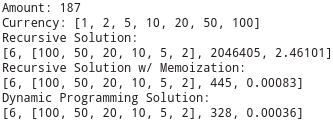
\includegraphics[width=2.9in]{../results/results_example.png}
    \caption{Console Output 1: algorithms execution example.}
    \label{code:1}
\end{figure}

\section*{3. Algorithm Complexities}

Let us now take a closer look at the theoretical behaviour of these functions.
The complexity of the algorithms' execution depends on 3 major factors, with the 
following characteristics, derived from experimental observations during
development: 
\setlist{nolistsep}
\begin{enumerate}
    \item The amount to be returned as change - the larger it is, the more coins
will have to be selected and the more combinations of coins can be chosen.
    \item The length of the currency array - the larger it is, the more coins 
available to be used as change have to be tested.
    \item The content of the currency array - depending on the available coins,
the algorithms might complete the task slower for some amounts.
\end{enumerate}

Taking this in consideration, it is easy to infer that finding an exact formula 
that determines the algorithms' complexities is far from trivial.
Nevertheless, with a formal analysis of the implementations, it seamed reasonable
that all solutions would have something similar to exponential growths in the 
number of basic operations as well as in execution times, although varying in 
the "speed" of growth.
But these were mere estimations and needed to be considered in greater depth.

For this reason, I resorted to an online tool that processes a set of values
given as input and returns a list of function approximations (through regression
analysis) that attempt to represent the behaviour of the input values.
Planetcalc \cite{planetcalc} received some coin amounts as X values and the
execution times and number of basic operations of each algorithm as Y values 
(once at a time) and estimated the regression functions that best fitted them.
The tested functions ranged from linear and quadratic regressions to hyperbolic,
logarithmic and exponential regressions. \\

The first conclusions drawned were that, for single-choice currencies (i.e. a 
currency array containing only the atomic unit), all algorithms behaved exactly
the same, with the number of basic occurrences given by $y=x$ and the execution
times approximately given by $y=ax$ for all algorithms, varying only the value
of 'a' in very small portions (in the scale of $10^{-6}$).
This means that, for such unique type of currency array, all algorithms have a 
complexity of $O(n)$.

Now, for all other currencies with more than one coin alternative, the 
behaviours diverged significantly.
While the algorithms with the use of stored values remained with a steady growth,
the recursive solution could clearly no longer be approximated with a linear 
regression and fitted best with an exponential one given by Planetcalc.
By passing to the online tool the amounts from 1 to 150 and the respective 
results relative to {\it tCMP\_recursive()\/}'s number of basic operations, and
after tweaking with the exponential regression's function approximation with 
the help of Desmos \cite{desmos} (an online graphical calculator) to fit it 
exactly with the practical results, I was able to reach the refined equation 
\ref{eq:3}:

{\setstretch{0.2}
\begin{equation} \label{eq:3}
    y = e^{7.00+0.0429x}
\end{equation}
}
Note that $y$ corresponds to the number of basic operations of the recursive 
algorithm, with $x$ as the change amount and a fixed currency of 
[1, 2, 5, 10, 20, 50, 100] (simulating the european currency, with the cents and 
the large bills ignored).
The currency was fixed in order to simplify the calculations; this currency was
used for the remaining calculations as well.
For different currency array sizes, the exponential approximation remained the 
best alternative, with larger arrays having a sharper exponential curve.
The same was true for same size arrays with different coin alternatives.

I then managed to estimate the complexity in Big-Oh notation by removing
constants from the formula and taking advantage of some mathematical properties 
of powers, as seen in equation \ref{eq:4}.
The result was a complexity of $O(1.04^{n})$.

{\setstretch{0.4}
\begin{equation} \label{eq:4}
    e^{7.00+0.0429x} \approx e^{0.0429x} = e^{0.0429^{x}} \approx 1.0438^{x} 
\end{equation}
}
Regarding the recursive with memoization and the dynamic programming algorithms,
the approach had to be different as, for the used amounts, the linear regression 
remained the best approximation for both.

Having an auxiliar matrix with the results of computations already calculated 
slows down the growth in execution time and total number of basic operations and
helps these algorithms be more efficient, but their internal functioning remains
the same, so I knew that their evolution was not linear.
So I ran the algorithms for larger amounts, up to 800 (since more than that
started reaching the maximum recursion depth of the Python language); then,
I used only a significant portion of the larger results on Planetcalc and
analysed the returned regressions.

After comparing individual representative values with the function 
approximations and removing negative constants (that would render the 
functions' y values lower than those constants meaningless), I reached the 
formulas that best fit {\it tCMP\_memoization()\/} and {\it tCMP\_dynamic()\/} 
respectively:

{\setstretch{0.2}
\begin{align} 
    y = 0.00012x^{2}+2.315x \label{eq:5} \\
    y = 0.00014x^{2}+1.655x \label{eq:6}
\end{align}
}

\newpage
I understood that the algorithms' complexities grew according to the amount 
(lets say 'n') and the currency array size ('m') (also according to the array's 
content, but its influence was small, so I ignored it for simplicity purposes) - 
this would result in a complexity of $O(nm)$. 
I also had in mind that any value for these two dimensions should be 
considered possible, so it was safe to consider 'n' as the largest of the two 
and derive from it a complexity of $O(n^{2})$.
Such complexity is typical of a quadratic function, so when choosing the best 
function approximations for the algorithms, I looked for a regression of that
nature. The outcome was equations \ref{eq:5} and \ref{eq:6}.

\section*{4. Performance Analysis}

In this chapter I explain the practical studies applied to the previously 
described algorithms.
Here, I execute each algorithm for different amounts and currencies.
I also describe the post-processing operations applied to the results to achieve 
more valuable conclusions. \\

The first thing done was presenting the results of running the algorithms for 
different amounts.
So, for each algorithm, several executions were done with amounts ranging from
0 to 150 (the later chosen for testing purposes, as larger numbers began to take
too long for the recursive solution).
This process was repeated for the following currencies: 
[[1], [1,2], [1,5], [1,2,5], [1,3,8,15,74,129], [1,2,5,10,20,50,100]].
These were chosen to evaluate the consequences of: increasing the size of the 
currency array, varying the coin alternatives for same size arrays, and choosing
coin alternatives with no direct relations.
The results of each execution were stored in a CSV file and printed in a 
formatted form similar to the one presented in Table 2 (see last page). \\

The next step was to visualize the results in order to better understand the 
performance for different inputs.
To do so, I used the library Matplotlib \cite{mpl}, a Python 2D library that 
produces figures in a variety of formats, and focused on the line plot.
The function responsible for generating the plots and storing them was
{\it tCMP\_generatePlot()\/}; it receives as arguments two lists, one containing 
the amounts tested, other containing the execution times of each algorithm for
each amount, it also receives the title of the figure, a smoothing factor and a 
logarithmic base.

The logarithmic base passed to {\it tCMP\_generatePlot()\/}, if greater or equal
to 2, is used to convert the time values into their logarithmic form.
The idea behind this was to allow the representation of all algorithms in the 
same plot, since the recursive grows a lot faster than the remainder and makes 
their visual analysis difficult, as seen in Figure 3.
However, applying this transformation did not influence much so it was not used 
in the studies considered in the remainder of this document.

\newpage
\vspace{-10pt}
\begin{figure}[H]
    \centering
    \setlength{\belowcaptionskip}{-10pt}
    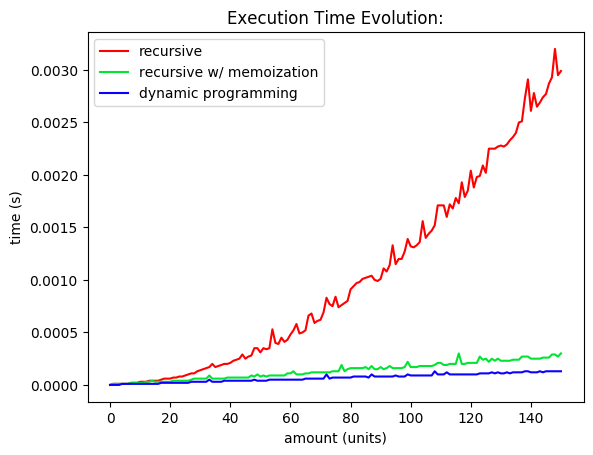
\includegraphics[width=2.9in]{../results/simple/tCMP_simple_results_plot_[15].png}
    \caption{}
\end{figure}
\vspace{-35pt}
\begin{figure}[H]
    \centering
    \setlength{\belowcaptionskip}{-10pt}
    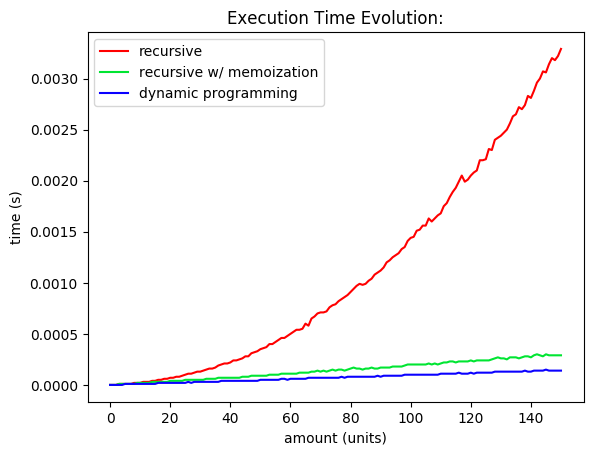
\includegraphics[width=2.9in]{../results/elaborate/tCMP_elaborate_results_plot_[15].png}
    \caption{Fig. 1, 2: Execution times of the 3 algorithms (single sequence and time averages of several sequences).}
\end{figure}

The smoothing factor, if larger than 1, is passed as argument to an auxiliar 
function {\it smooth\_results()\/} responsible for, as the name states,
smoothing the results.
The way this works is by collecting groups of 'x' values from the execution 
times list and calculating the average value between them.
Here, 'x' is given by the smoothing factor passed as argument.
The sampling set is then reduced 'x' times, making the plot quicker, with less
irregularities but with less detail as well.
This smoothing process was also not used, as a better alternative was found.

These irregularities, or noise, correspond to small time rises during execution 
that negatively influence times spent in calculations in a way that does not 
represent the reality of the algorithms.
What I mean is that, for external reasons other than the actual functioning of 
the developed functions, occasional time peaks occur for different executions.
This was detected as these peaks occur in different places when the functions 
are executed several times with the same input.
This noise is visible in Figure 1. \\

The solution developed that tackles this issue better than the smoothing process
was to run the set of input combinations several times and calculate the average
execution time of each combination.
Figure 2 shows the plot of the execution of the algorithms for the 
same input values as of Figure 1, but doing so 50 times and 
calculating the averages, hence removing most of the noise. This value was 
chosen by trial and error, as beyond 50 the amount of noise removed did not 
compensate the additional amount of time required to execute the study.

The two plots correspond to executing the algorithms for values from 0 to 150,
with a currency array of only two coins [1,5]. 
But what if this array increases?
Figures 3 and 4 show what happens when we execute the
algorithms for a currency of [1,2,5,10,20,50,100].

Both figures present the average times of running the procedure 50 times like we
saw in Figure 2, and correspond to the exact same run, differing only 
in the fact that in the second plot the recursive values are not presented so 
that we can better analyse the others.

\begin{figure}[H]
    \centering
    \setlength{\belowcaptionskip}{-10pt}
    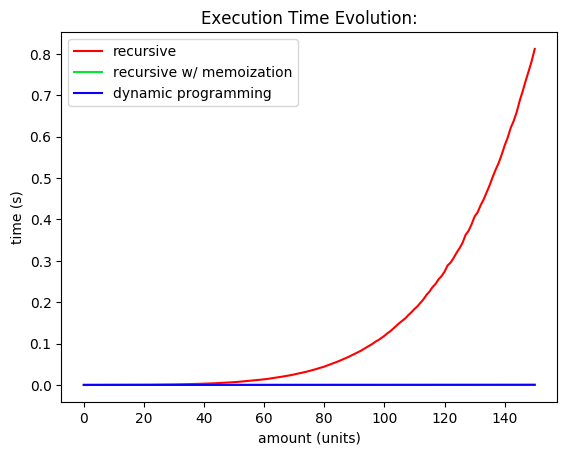
\includegraphics[width=2.9in]{../results/elaborate/tCMP_elaborate_results_plot_[125102050100].png}
    \caption{}
    \label{fig:3}
\end{figure}
\vspace{-25pt}
\begin{figure}[H]
    \centering
    \setlength{\belowcaptionskip}{-10pt}
    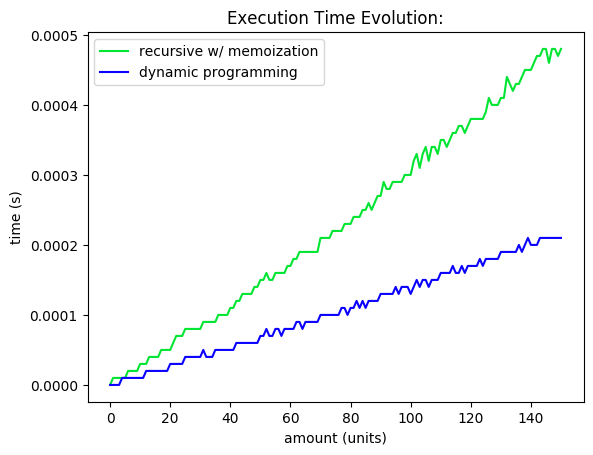
\includegraphics[width=2.9in]{../results/elaborate/tCMP_elaborate_results_plot_[125102050100]_memory.png}
    \caption{Fig. 3, 4: Execution times averages of the 3 algorithms (for a larger currency array).}
    \label{fig:4}
\end{figure}

Through the plots, one can conclude that the function approximations seem
adequate to the behaviours of all three algorithms.
It is also visible the fact that the larger the number of available coins, the
sharper is the growth curve of the recursive algorithm, while the others remain 
very much stable.

Testing the algorithms for currencies with coins without clear patterns (e.g. 
having coins that are multiples of each other) proved to have no noticeable 
effect on the results.

\begin{comment}
One additional question I placed during these tests was wether or not choosing 
currencies with coins without clear patterns (e.g. having coins that are 
multiples of each other) would affect the behaviour of the algorithms.
Figure 5 shows the plot of testing them for a currency of 
[1,3,8,15,74,129]. For all intents and purposes, if this has any consequence 
whatsoever, it was not noticeable for the enforceable tests.

\begin{figure}[H]
    \centering
    \setlength{\belowcaptionskip}{-10pt}
    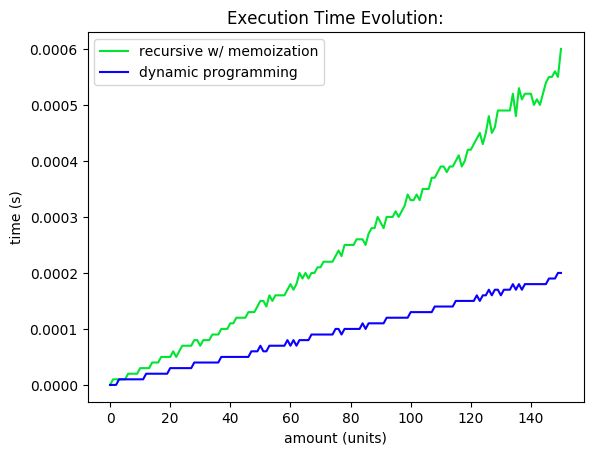
\includegraphics[width=2.9in]{../results/elaborate/tCMP_elaborate_results_plot_[1381574129]_memory.png}
    \caption{}
    \label{fig:5}
\end{figure}
\end{comment}

\newpage
\section*{5. Algorithm Comparisons \& Additional Considerations}

In this final chapter, I compare the three developed algorithms in terms of 
complexity, execution time, memory usage and readability and present the 
gathered conclusions.
Finally I present a reasoned prediction of the algorithms behaviour for 
significantly larger amounts, with the help of regressions, and mention a few 
additional considerations worth stating. \\

It is needless to say that, of the three algorithms, the slowest and less 
adviseable is the recursive without memoization.
This algorithm, although elegant as most recursive functions are, is not 
scaleable at all as it is constantly repeating computations it has already made
before.
As for the other two, from the analysis previously made, it is concluded that 
the recursive with memoization is usually twice as slow as the dynamic.
This is due to the fact that recursive calls are inherently slower than an 
iterative loop.
But the small implementation differences might also have an impact that benefits
the dynamic programming solution.

In terms of readability, {\it tCMP\_dynamic()\/} has the advantage as well, 
since it contains less verifications.
The only aspect in which {\it tCMP\_recursive()\/} is better than the others is
in terms of reduced memory usage, obviously, as it does not keep track of any 
variable other than the ones strictly necessary. \\

For a final and hypothetical exercise, I present an estimation of the execution
times of the three algorithms for amounts equal to $10^{3}$, $10^{6}$ and $10^{9}$ .
This is ment to illustrate how big can be the consequences of not searching for
efficient and scalable solutions, and resorts to the regressions presented in 
chapter 3 (see equations \ref{eq:3}, \ref{eq:5} and \ref{eq:6}) to provide with
the estimations.
Note that these equations return an estimation of the total number of basic 
operations of each algorithm given an amount; in order to use them, we need to
convert the results into execution times; this is easily done by finding the 
relation between basic operations and execution times.
Once again, Planetcalc helps in finding these relations.
For the recursive solution, the execution time is 1.1767 x $10^{-6}$th of the 
total number of basic operations; for the recursive with memoization, it is
1.3546 x $10^{-6}$th; and for the dynamic programming it's 0.8164 x $10^{-6}$th.
The results are visible in Table 1.

\begin{figure}[H]
    \centering
    \setlength{\belowcaptionskip}{-10pt}
    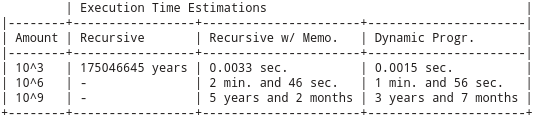
\includegraphics[width=3.3in]{../results/results_estimations.png}
    \caption{Table 1: Execution time estimations derived from the function approximations.}
    \label{tab:1}
\end{figure}

\newpage
The estimations greater than $10^{3}$ are not presented for the recursive 
algorithm as their values were ridiculously big, tending to infinity.
The other two proved to be very robust algorithms, given that, even for an amount
of a billion to return as change, they could complete the task in less than 
10 minutes. \\

I end this report with a few final considerations.
Regarding shortcomings of my work, I have two aspects to mention.
The fact that the recursive algorithms quickly reached Python's maximum 
recursion depth was unfortunate, but my efforts of avoiding such limitation
were not as effective as would be desired.
Also, the differences between the matrices of {\it tCMP\_memoization()\/} and 
{\it tCMP\_dynamic()\/} and the way they are manipulated was an aspect to 
overcome in the event of continuing the work, as it would probably demand for
changes in all three algorithms.
I would like to mention that, although the algorithm implementations were 
developed by me, most of the reasoning behind was taken from several sources 
combined, in order to attempt to deliver the code as best optimized as possible.

The entire code is present in the file {\it TheChangeMakingProblem.py\/},
with a few execution examples in the end.
I make available a {\it requirements.txt\/} file containing the dependencies
for the execution of the code.
The functions and some important code lines have comments to help guide myself
during development and a potential reader henceforward.
Along with this document and the source code, I also deliver a results folder 
containing all of the plots presented here and a few more with different variable
combinations.

\bibliography{report.bib} % use a field named url or \url{} for URLs
% Note: the \bibliographystyle is set automatically

\newpage
\begin{figure*}[ht]
    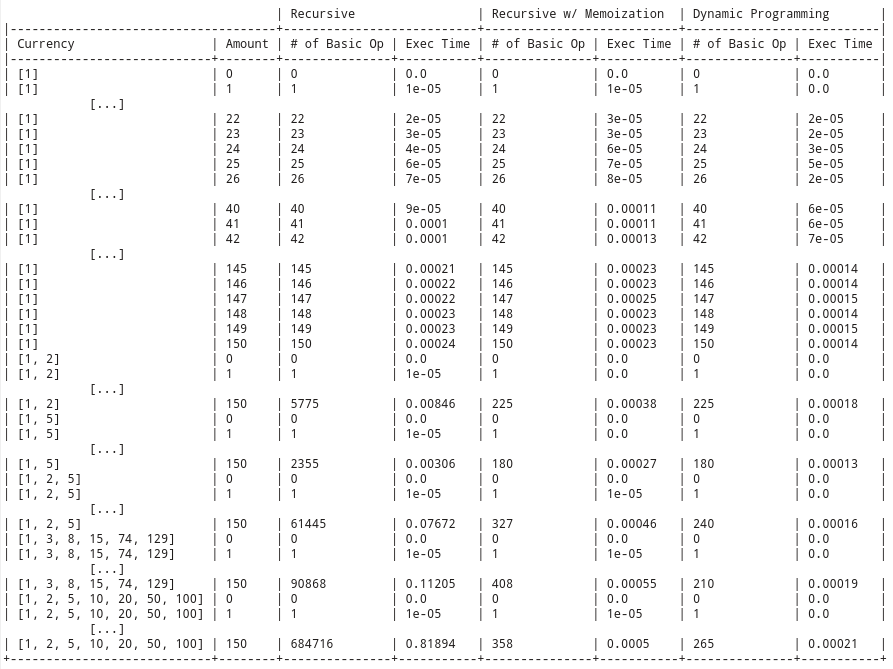
\includegraphics[width=\linewidth]{../results/results_table.png}
    \caption{Table 2: Portion of the output of a simple study of the algorithms.}
    \label{tab:2}
\end{figure*}

\end{document}
